\chapter{Human MS-based Protein expression landscape}\label{ch:proteomics}

\setlength{\epigraphwidth}{0.7\textwidth}
    \setlength{\epigraphrule}{0pt}
    \epigraphhead[5]{%
    %\epigraph{\emph{On m'a enseigné que la voie du progrès
    %n'était ni rapide ni facile.}}{Marie Curie}
    \epigraph{\emph{I was taught that the way of progress is
    neither swift nor easy.}}{Marie Curie}
}

After exploring the high-throughput human transcriptomic studies
in \Cref{ch:Transcriptomics}
and before integrating them with proteomic data in \Cref{ch:Integration},
I present in this chapter the comparison of
the three proteomic datasets introduced in \Cref{ch:datasets}.
\citet{Ezkurdia2014-qx,Deutsch2015} have partially reviewed these data.
However, we have reprocessed them starting from the raw data
for this thesis.
In this context, reassessing the quantified processed proteomic data
before any integration is pertinent.\mybr\

The work presented in this chapter was done in collaboration with \james\
who has implemented the new protein quantification method
(presented in \Cref{sec:NewQuantProt}).
I have received general feedback from \alvis, \mar,
\sarah\ and Faranak Ghahreman.
A manuscript describing part of this chapter's work
and the one presented in \Cref{ch:Integration} is being prepared.\mybr\

\section{An~overall~fragmented~and~disparate~universe~to~explore}

As I have described in \Cref{ch:background},
proteins present a wide range of physicochemical properties
(see \Cref{sec:bio} and \Cref{sec:aa})
and are challenging to identify and quantify
in high-throughput studies (see \Cref{sec:exploreProtMS}).
Thus, it comes as no real surprise that
while the use of \ms\ for proteomics has been developing since the 1980s~\mycite{BiomolBio},
the first notable attempts to draft the human proteome occurred only recently
in 2014~\mycite{PandeyData,KusterData},
or that the oldest (unpublished) available multi-tissue \cutler\ dataset is from 2010
(see \Cref{subsec:cutler}).
To this date,
\cutler Lab, \kuster\ Lab and \pandey\ Lab datasets are the only ones
that explore concurrently several nondiseased human tissues.
See \Cref{sec:ProteoData} for more details and
the processing pipeline designed and implemented by \james\ to handle them.\mybr\

As presented in \Cref{fig:VennDiagProt3},
they share four tissues: \heart, \lung, \ovary\ and \pancreas.
The protein overlap of this four-tissues set between these three datasets
is rather narrow as shown in \Cref{fig:VennProtComm}.
The \cutler\ Lab dataset is the most limiting factor;
\pandey\ Lab and \kuster\ Lab datasets share over twice as many proteins
that they share with \cutler\ (3,338 instead of 1,384).
The number of shared proteins between \pandey\ Lab and \kuster\ Lab data rise to 4,172
when all their fourteen common tissues are considered.\mybr\

\begin{figure}[!htpb]
    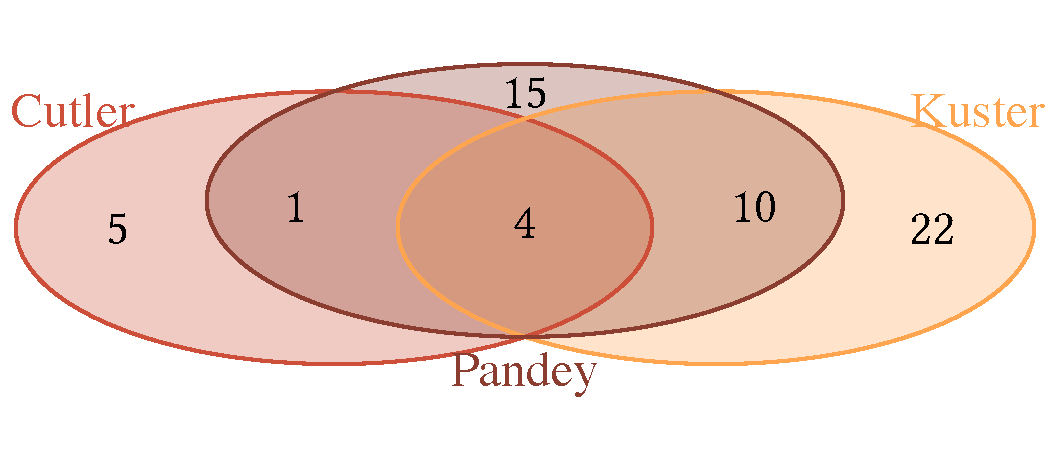
\includegraphics[scale=0.71]{proteomics/VennDiagProtCond.pdf}\centering
    \vspace{-5mm}
    \caption[Distribution of unique shared tissues between
    the 3 MS-based proteomic studies]{\label{fig:VennDiagProt3}\textbf{Distribution
    of unique and shared tissues between the three MS-based proteomic studies.}
    The three datasets share together: \heart, \lung, \ovary\ and \pancreas.
    The two most recent studies share fourteen tissues in total;
    the additional ten tissues are: \adrenal, \hcolon, \gallbladder,
    \oesophagus, \kidney, \liver, \placenta, \prostate, \rectum\ and \testis.}
\end{figure}
%\vspace{1cm}
\begin{figure}[!htpb]
    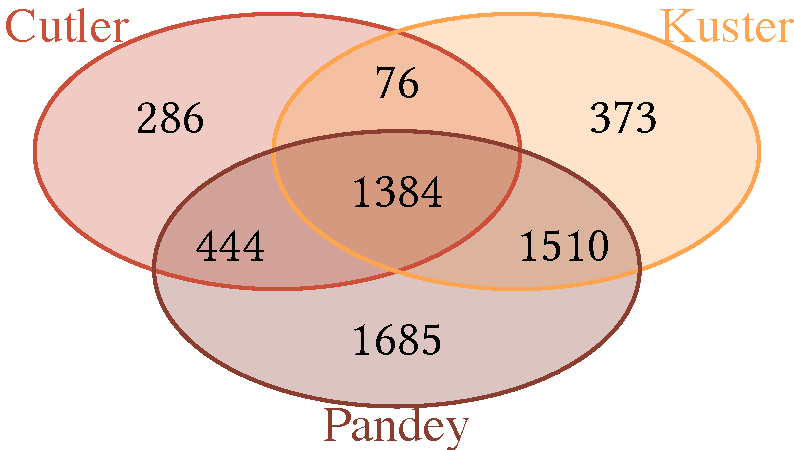
\includegraphics[scale=0.75]{proteomics/VennDiagProtFor4T.pdf}\centering
    \vspace{-5mm}
    \caption[Proteins overlap between the common tissues of
    the 3 proteomic studies]{\label{fig:VennProtComm}\textbf{Proteins
    overlap between the common four tissues of the three proteomic studies.}
    Unique and shared proteins detected and quantified
    across the three \ms\ studies for their four shared tissues:
    \heart, \lung, \ovary\ and \pancreas.}
\end{figure}
\clearpage
\subsection{High-throughput MS proteomic data has high detection variability}

\Cref{fig:barplot3Dvennprot}
illustrates the number of proteins identified in each of these four tissues.
The colours indicate in which dataset (or group of datasets)
the proteins have been identified.
See \Cref{fig:protbkdownT} for each set precise numbers.\mybr\

\begin{figure}[!htbp]
    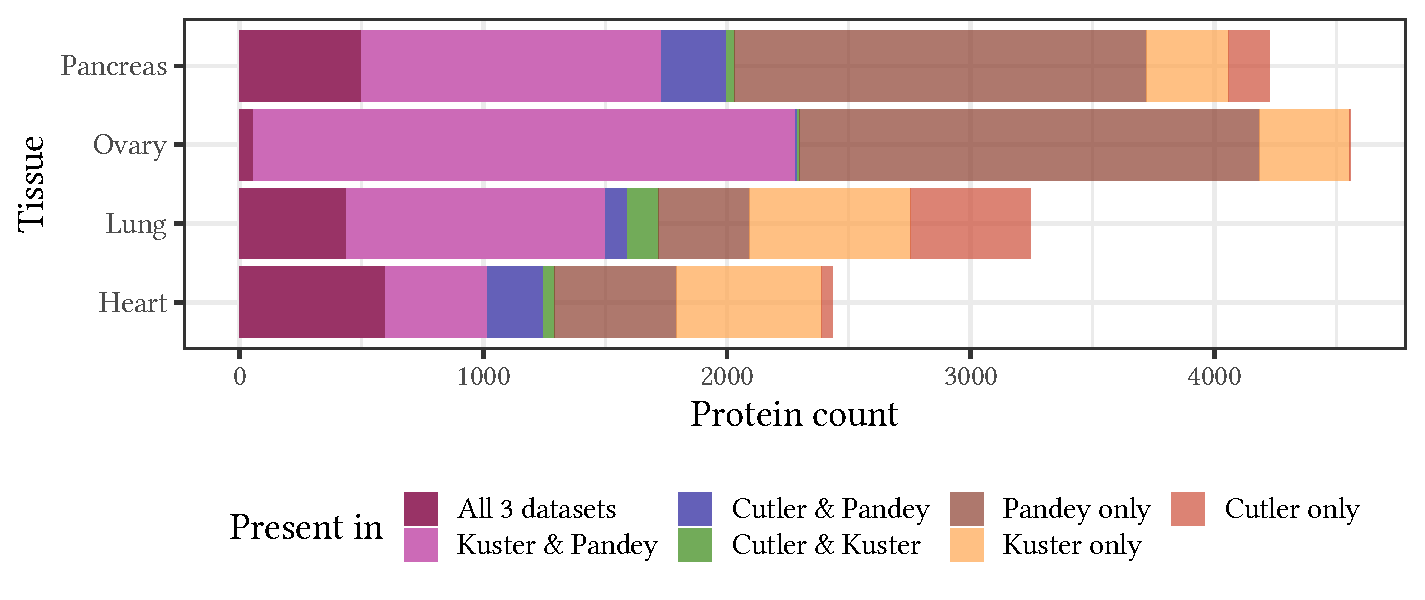
\includegraphics[scale=0.65]{proteomics/barplotVenn3Dprot.pdf}\centering
    \vspace{-3mm}
    \caption[Identified proteins across the 4 shared tissues for the 3 datasets]%
    {\label{fig:barplot3Dvennprot}\textbf{Number of identified
    proteins in each of the four common tissues for the three proteomic data.}
    Proteins found in more than one dataset are most likely true (in
    red, light and darker green or purple --- the most validated ones in red
    as they are found in all three datasets).
    See \Cref{fig:protbkdownT} for the precise numbers in each set.}
\end{figure}

The tissue with the highest number of identified proteins,
regardless of which dataset,
is the \ovary.\mybr\

The highest number of proteins identified in all three datasets at once (600)
is in the \heart.
The other tissues have
the \emph{Kuster and Pandey} set as
their largest protein group formed by more than one dataset.\mybr\

The largest set of identified proteins in \pancreas\
and the second one in \ovary\ are proteins only found in \pandey\ Lab dataset
(\emph{Pandey only}).
As shown in \Cref{fig:distribProtUniq3D},
our pipeline has identified the highest number of proteins in the \pandey\  Lab dataset.
Thus, it is coherent that \pandey\ Lab proteins represent a large part of
the identified proteins in each tissue (either as \emph{Pandey only} set or
in agreement with the other datasets:
\emph{All 3 datasets}, \emph{Kuster \& Pandey} or \emph{Cutler \& Pandey}).
More surprising is that the \cutler\ dataset comprises a respectable amount of
proteins in \lung\ that are missing in the other two.
A few of these proteins (82) are missing altogether,
but a subset of them (410) is still found
in (at least) another tissue of the other datasets.\mybr\

\begin{figure}[!htpb]
    \includegraphics[scale=0.8]{proteomics/ProteinUniqueDistribPerdatasets.pdf}\centering
    \caption[Distribution of the proteins per tissue]{\label{fig:distribProtUniq3D}%
    \textbf{Distribution of the proteins per tissue across the three datasets.}
    \cutler\ Lab dataset has the smallest and \pandey\ Lab the highest number of proteins
    per tissue.
    Coloured in red are the proteins that have uniquely been identified
    in one tissue (or cell type) in each dataset;
    in turquoise are proteins that have been identified in several samples
    of the dataset.}
\end{figure}

While proteins found in more than one dataset are more likely true positives,
it is impossible to exclude without risks the ones
that are identified in one dataset only.
Whether an identified protein in one dataset is
an artefact (\ie\ false positive) or a miss (false negative) in the other datasets
is a challenging question;
the diversified nature of proteins involves
many sample preparation and simplification methods
(see \Cref{subsec:ProtSampPrep,subsec:simpleProt}).\mybr\



%\vspace{-0.5cm}

\subsection{About half of the identified proteins are found in the same tissue
in different datasets}\label{subsec:halfProtConfirmed}

As shown in \Cref{fig:barplot3Dvennprot,fig:protbkdownT,fig:protbkdownT10more},
besides a few exceptions (\oesophagus, \gall\ and \testis),
more than half of the proteins are identified in the same tissue
in more than one dataset.
Three proteins are found in every tissue of every dataset:
\protein{ALB},  \protein{KRT9}, \protein{KRT10}.
This number rises to forty when only the \pandey\ Lab and the \kuster\ Lab data
are considered (see \Cref{tab:ubiProt2D}).
I have also investigated tissue-specific (\gls{TS}) proteins
(in red in \Cref{fig:distribProtUniq3D})
that are also identified in more than one dataset.
While the three datasets lacked to identify any \gls{TS} protein at once,
\pandey\ Lab and \kuster\ Lab datasets share a few (44 across eight tissues)
--- see \Cref{tab:comTSprot} for the complete list.\mybr\
\begin{comment}
twelve for \kidney, nine for \placenta, seven for \pancreas,
five for \adrenal\ and \liver, four for \testis,
and one for \prostate\ and \rectum.
\end{comment}

\gls{TS} proteins are more difficult to confirm
through different datasets,
but one needs to be careful with the ubiquitous proteins as well.
The latter may be present in the samples due to contamination:
none of the three ubiquitous proteins
(\protein{ALB},  \protein{KRT9} and \protein{KRT10})
is detected in \heart\ by the
\hFo{Human Protein Atlas}{https://www.proteinatlas.org/}~\mycite{Uhlen2015}
while they are found in epithelial cells.
One hypothesis is that contamination occurred when sampling from the donor.\mybr\

Lists for ubiquitous and \gls{TS} proteins of each dataset separately
and across the three (when consistent) are given as digital supporting data.\mybr\

\vspace{-3mm}

\subsection{Technical variability prevails over biological signal:
intrastudy correlations of different tissues are globally stronger than
same-tissue interstudy correlations.}\label{subsec:protTechVarHigh}


After defining the (1,384) protein set that is consistently detected
in the four common tissues of the three datasets,
I have assessed how consistent is
their expression quantification across tissues and studies.\mybr\

\begin{figure}[!htbp]
    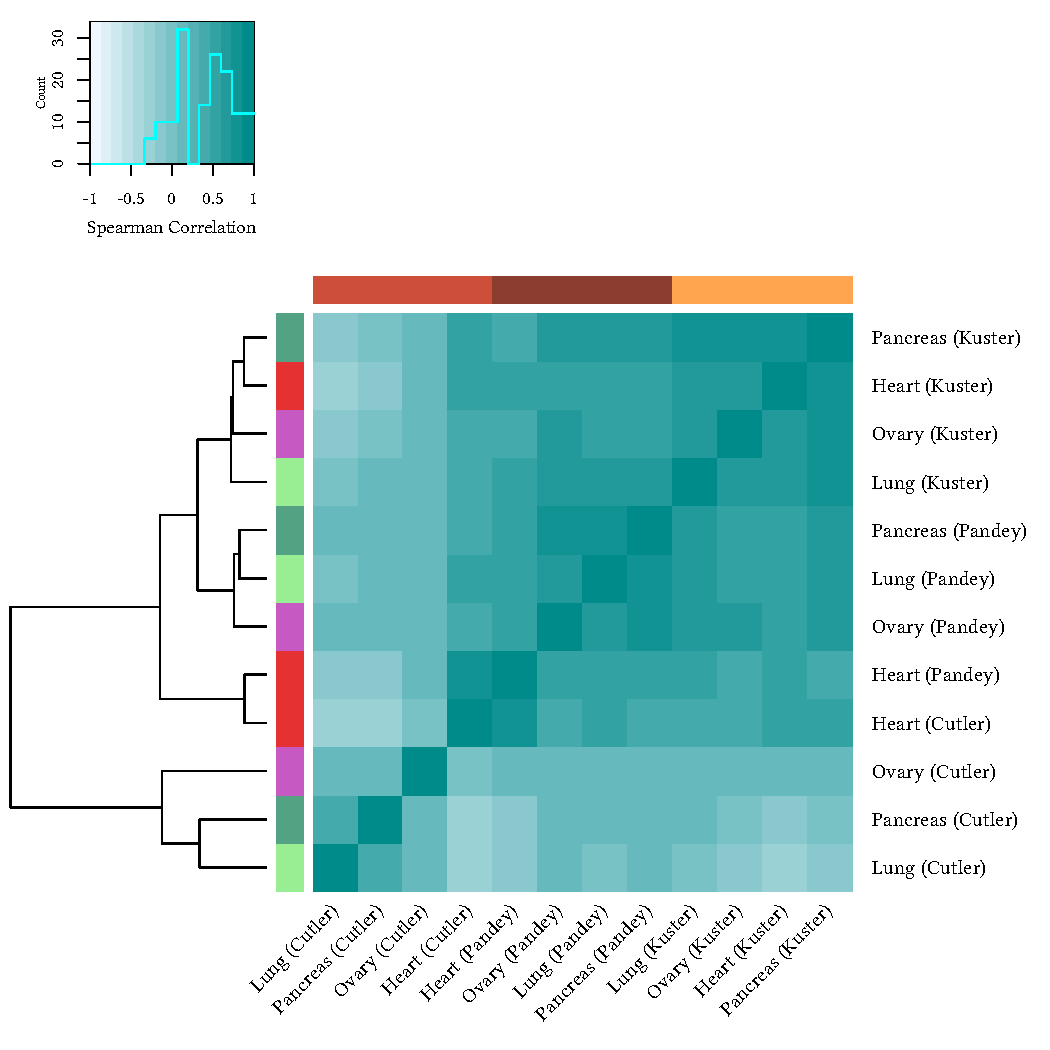
\includegraphics[scale=0.9]{proteomics/heatmap3DproteinSpearman.pdf}\centering
    \caption[Heatmap of the four common tissues between the three proteome
    datasets]{\label{fig:prot3Dheatmap}\textbf{Heatmap of the four common tissues
    between the three proteome datasets} based on
    the pairwise Spearman correlations clustering of 1,384 proteins expression levels.
    Only \heart\ from \cutler\ Lab and \pandey\ Lab have a stronger intratissue correlation
    than an intrastudy one.
    Both for \pandey\ Lab and \cutler\ Lab,
    \pancreas\ and \lung\ are more correlated to each other and their pair to \ovary.
    The heatmap (\Cref{fig:prot3DheatmapPears})
    based on Pearson correlation instead prompts globally identical observations.
    See also \Cref{fig:scat3DheartCutlerPandey} that shows (as a scatterplot)
    the relationship for \Heart\ between \pandey\ Lab and \cutler\ Lab, and then,
    \Cref{fig:scat2DPlacentaKusterPandey} between
    \pandey\ Lab and \kuster\ Lab.
    }
\end{figure}

Following a similar approach to \Crefp{fig:noMitoNoRep4T},
I cluster the twelve proteomic \treps\footnote{See~\Vref{def:trep} for \treps\ definition.}.
I have used Ward's method to link the \treps\ based on their similarity that
I have computed by substracting from 1 the pairwise Spearman correlation
of the expression levels of the 1,384 common proteins.
As shown in \Cref{fig:prot3Dheatmap},
the technical variability overcomes the biological signal
as the proteomic \treps\ cluster according to their original laboratory/study
rather than their biological source,
except for \cutler\ Lab and \pandey\ Lab \heart.
However,
\cutler\ Lab and \pandey\ Lab share the same organisation of their remaining tissues:
\pancreas\ and \lung\ are the most correlated,
and their pair is in turn most correlated to \ovary.
\kuster\ Lab \treps\ display the greatest amount of study bias
(probably due to stronger batch effects --- see \Cref{sub:BatchEffect}).\mybr\

Removing the proteins translated from the mitochondrial genes slightly
improves the results
but excluding the three ubiquitous (likely contaminants) proteins, presented
in \Cref{subsec:halfProtConfirmed},
is impactless.\mybr\

Because of the limited number of proteins included in this analysis,
it is unwise to draw definite conclusions
except that there is an extensive need for new quantification normalisation methods
that can help with protein expression meta-analyses
and as for now one has to be very cautious when comparing proteome samples.\mybr\

I attempted to expand this analysis by comparing the fourteen common tissues
of \pandey\ Lab and \kuster\ Lab datasets,
but the results are as inconclusive
(see \Cref{fig:prot2DheatmapT14,fig:prot2DheatmapPearson}).\mybr\

\section{New quantification method}\label{sec:NewQuantProt}

In this thesis context where I aim to integrate
the \mRNA\ expression levels to the protein ones
(presented in \Cref{ch:Integration}),
I have developed a new method to infer and quantify the proteins
with the help of \james.\mybr\

Our original processing workflow (detailed in \Cref{subsec:msDataProcess})
intends to provide a reliable protein quantification.
Our method seems more rigorous than \citet{PandeyData} original paper;
\citet{Ezkurdia2014-qx} challenge the correctness of their quantification
by highlighting the disputable presence of \glspl{OR} in many tissues.
On the other hand, our workflow lacks to detect or quantify any possible \gls{OR}
in the \pandey\ Lab data.
The left part of \Cref{fig:newQuantProtMeth} summarises
our first method of quantification.\mybr\

\begin{figure}[!htbp]
    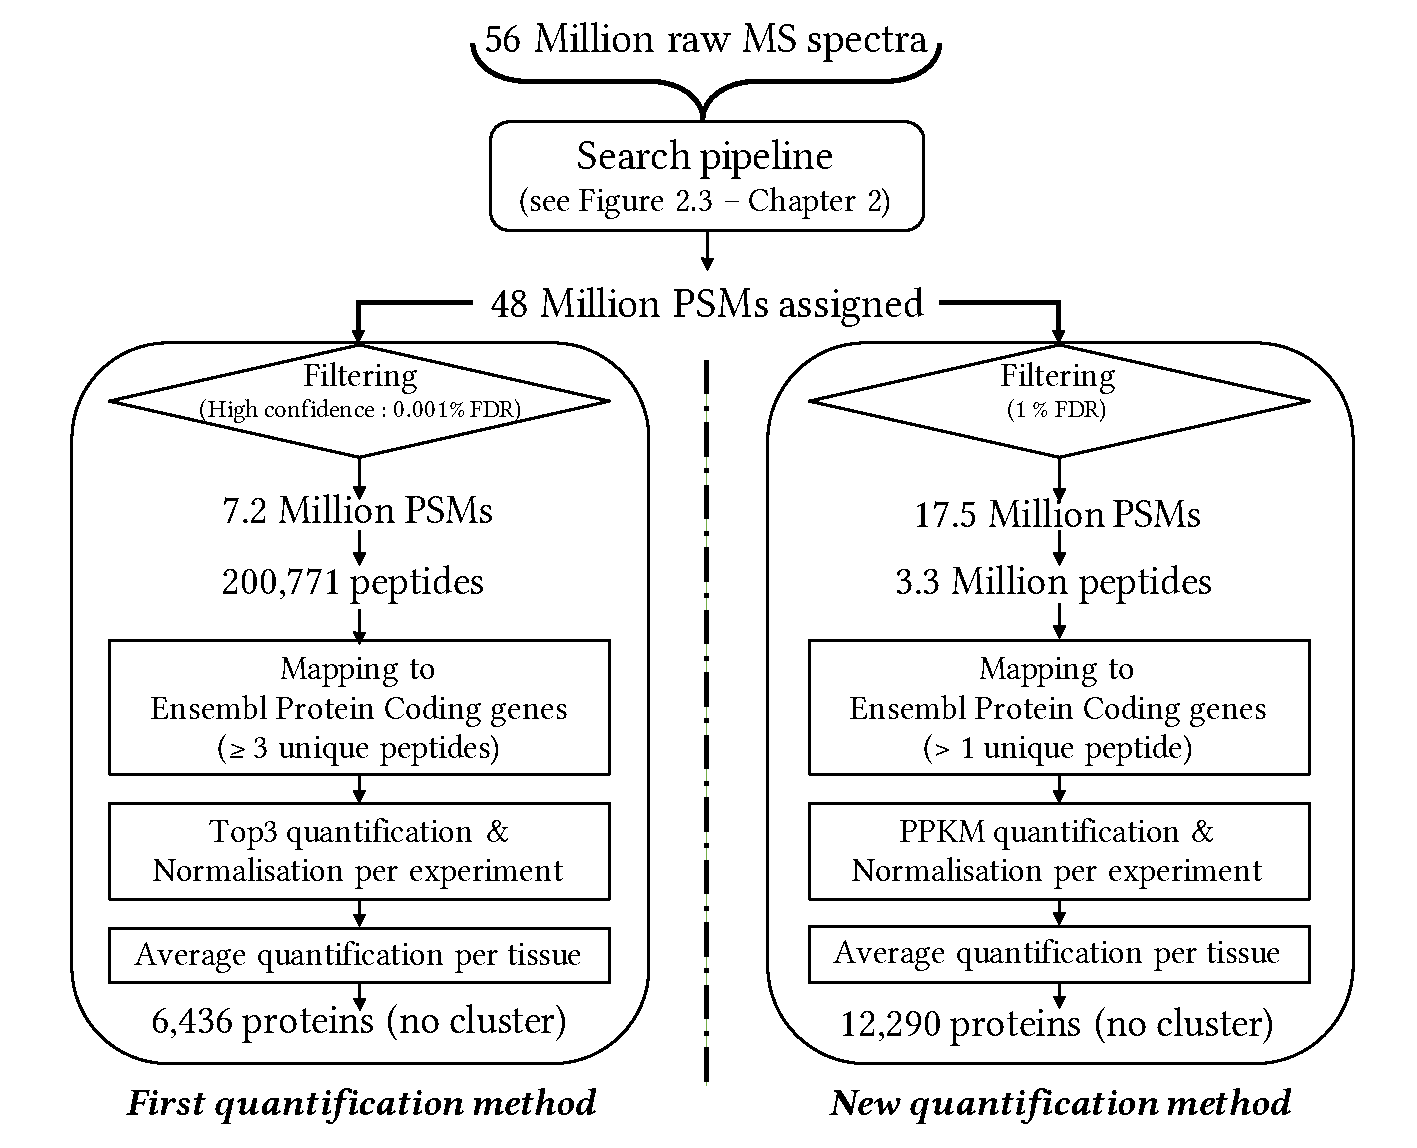
\includegraphics[scale=0.7]{proteomics/quantificationQ1Q2.pdf}\centering
    \caption[Two quantification methods for Pandey Lab data]{\label{fig:newQuantProtMeth}\textbf{Two
    quantification methods for Pandey Lab data.}
    For both approaches, the search pipeline assigning \psms\ remains identical
    (see \Cref{subsec:msDataProcess}).
    The first quantification method,
    which follows a robust inference method
    involving at least three unique peptides,
    relies on the intensity of the three most intense unique peptides.
    The new quantification method that I have invented
    allows more relaxed inference parameters
    as it also uses the non-unique peptides for the quantification.
    See \Cref{eq:PPKM},
    which is similar to \Vref{eq:rpkm-fx}.
    After averaging per tissue and removing the clusters,
    the number of quantified proteins with the new method
    is close to twice the number provided by the first described method.
    The new quantification method was designed
    for the analyses in \Cref{ch:Integration} in particular;
    this is why the filtering is also less strict than for the first quantification method
    since my main focus is the integration of the proteomic data
    with the \Rnaseq\ data.
    Clusters are protein groups that can be mapped to
    more than one \gls{Ensembl} gene identifier.
    Note that the final proteins numbers include only the fifteen tissues
    used for the integration in the following \Cref{ch:Integration}.
    }
\end{figure}

While probably more accurate,
our first quantification is also more stringent than the original one.
Thus, the total number of quantified proteins is more limited.
The requirement of three unique peptides to identify and quantify the proteins
appears to me as the obvious main limiting factor of our method.
As presented in \Cref{ch:background},
the protein quantification relies on
\psms\ identification (see \Cref{subsub:peptideID})
and the chosen approach to infer the proteins (see \Cref{subsec:proteinInference}).
Our first method infers proteins from sets that comprise at least three unique peptides.
The quantification relies on a Top3 approach~\mycite{Silva-Top3}.
It uses the three \emph{unique} most expressed peptides of a protein
to estimate its overall expression
(see \Cref{eq:Top3} (\vref{eq:Top3}) and \Cref{subsubsec:protQuantLB}).\mybr\

\begin{minipage}{\textwidth}
\begin{equation}
    \tag{Top3 \gls{IBAQ}}\label{eq:Top3}
    \hat{\mu}_{ij}=\frac{\sum \text{Intensity of Top 3 unique peptides} _{ij}}{\text{Total Intensity in experiment } j}
    \raisetag{3\normalbaselineskip}
\end{equation}

where:{\small
\begin{itemize}[topsep=0pt,nosep]
    \item $\hat{\mu}_{ij}$ is the normalised expression for the protein $i$ in experiment $j$ (normalised \gls{PSM}),
    \item $\sum \text{Intensity of Top 3 unique peptides} _{ij}$ is
        the sum of the intensity of the three most intense unique peptides
        of the protein $i$ (mapped to its gene definition $G_i$),
    \item $\text{Total Intensity in experiment } j$ is the total sum of the intensity of all
the peptides identified in the experiment $j$.
\end{itemize}
}
\end{minipage}

The new method I have devised uses both the unique and
the \emph{degenerate} (\ie\ non-unique) peptides
for the quantification step.
It allocates the degenerate peptides
in proportion to the distribution of unique peptides per protein
following a similar approach to \cuffl\ for \Rnaseq\ data (see \Cref{minisec:Cufflinks}).
As three unique peptides are no longer required for the quantification,
it allows relaxing the inference parameters to two unique peptides
(in order to still avoid \emph{one-hit wonders}, see \Cref{subsec:proteinInference}).
The new quantification follows a similar approach to the \RPKM\ normalisation ---
see \Cref{eq:rpkm-fx}.
Protein expression levels are expressed in \glspl{PPKM},
which stands for \glspl{PSM} Per Kilobase of gene per Million.\mybr\

As shown in \Cref{eq:PPKM},
this method counts the number of \psms\
that can be mapped to the corresponding \gls{Ensembl} gene identifier of a protein.
Then, this raw count is normalised by dividing it
by the product of the longest transcript length and the total number of \psms\
assigned in that experiment;
the result is finally multiplied by a factor ($10^6$) to facilitate reading.
Using the longest \emph{transcript} length
instead of the longest protein isomer allows avoiding issues due to
annotation differences between gene and protein levels
in the analyses of the following \Cref{ch:Integration}.\mybr\

\james\ has implemented this new method and provided me
\PPKM\ quantifications for the \pandey\ Lab data.\mybr\

\begin{minipage}{\textwidth}
\begin{equation}\label{eq:PPKM}
    \tag{PPKM definition}
    \hat{\mu}_{ij} = \frac{\text{Number of \psms\ matching } G_i \cdot10^{-6}}{\ell_{G_i}\cdot\sum \text{\psms}_j}
\end{equation}

where:{\small
\begin{itemize}[topsep=0pt,nosep]
    \item $\hat{\mu}_{ij}$ is the normalised expression of the protein $i$
        in the experiment $j$,
    \item $\text{Number of \psms\ matching } G_i$ is the number of \psms\ mapped
        to the definition of the gene $G_i$ that corresponds to the protein $i$,
    \item $\ell_{G_i}$ is the length of the longest transcript of the gene $G_i$,
%\text{Longest transcript length for } G_i$
    \item $\sum \text{\psms}_j$ is the total number of \psms\ identified in
the experiment $j$.
\end{itemize}
}
\end{minipage}

Although smaller,
another limiting factor is the filtering threshold of the selected \psms\
to be inferred in proteins.
We have chosen a conservative (and state-of-the-art) threshold prior to
the first quantification filtering
and a less strict one for the new method.
As my aim is to compare and integrate proteomic and transcriptomic data together,
an increased number of false positives among the identified proteins
(see \Cref{subsub:peptideID}) is not a real issue.\mybr\

\begin{figure}[!htbp]
    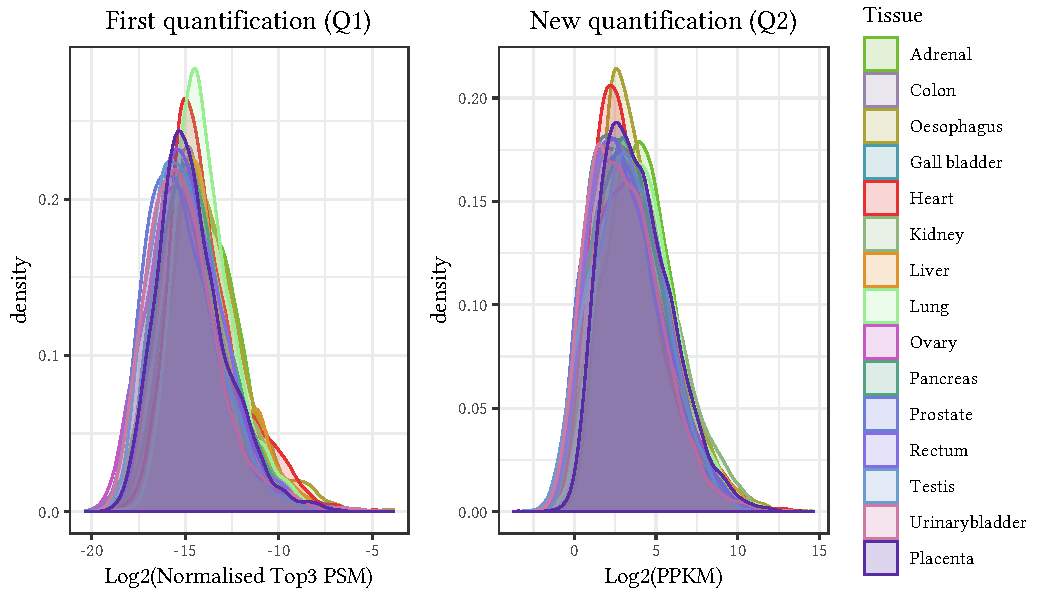
\includegraphics[scale=0.7]{proteomics/distribPandeyQ1Q2.pdf}\centering
    \vspace{-2mm}
    \caption[Pandey Lab data protein expression distribution
    with two quantification methods]{\label{fig:pandeyDistribQ1Q2}\textbf{Distribution
    of the protein expression levels with two different methods.}
    On the left, the protein expression levels distribution for the adult
    tissues of the \pandey\ Lab data with our first quantification method
    (described in \Cref{subsec:msDataProcess}).
    This figure is similar to \Cref{fig:distribProt}(c) but without the fetal tissues.
    On the right are the protein expression levels of the same tissues that
    have been computed with the new quantification method.
    The overall shape of the density plots is very similar between the two approaches.
    }
\end{figure}

Before moving on to the integration of the proteomic and transcriptomic data
in the next chapter,
I have carried out a few comparisons
between the first and the new quantification methods.
As shown in \Cref{fig:pandeyDistribQ1Q2},
the densities of distribution of protein expression levels per tissues
have similar shapes between the two methods.\mybr\

\Cref{fig:pandeyQ1Q2comp} presents the number of quantified proteins per tissue.
The new method allows quantifying for some tissues
up to more than twice the number quantified by the first method.
This proportion is consistent with the total number of proteins identified
across the fifteen adult tissues
by the first method (6,436)
and the new one (12,290).\mybr\

\begin{figure}[!ht]
    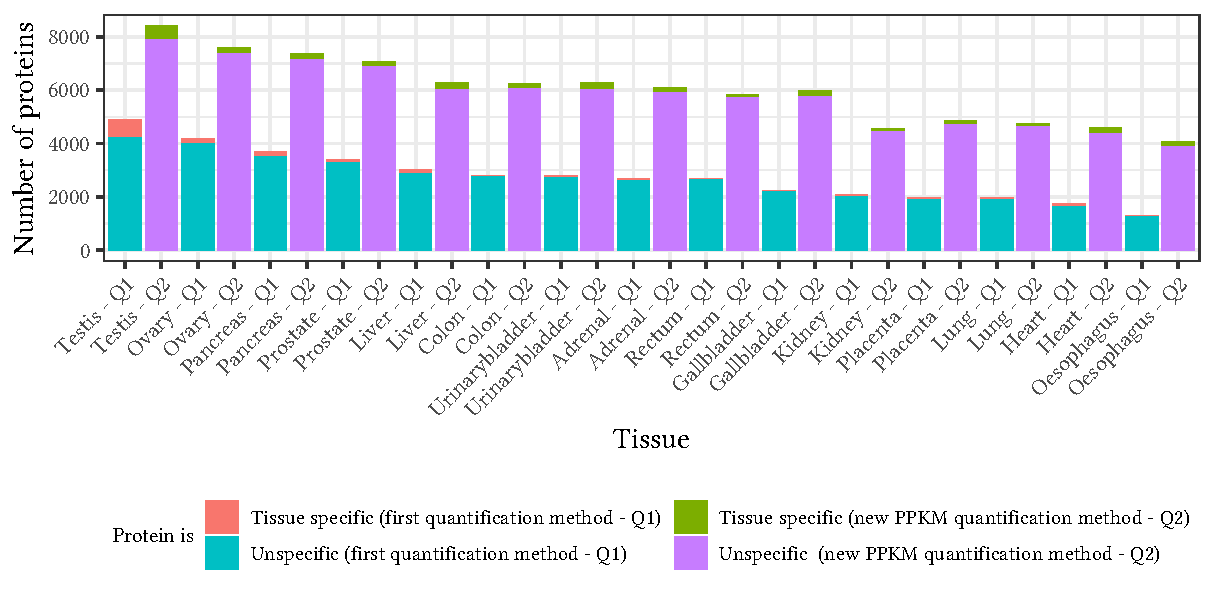
\includegraphics[scale=0.82]{proteomics/compDistribQ1Q2pandey.pdf}\centering
    \vspace{-3.5mm}
    \caption[Comparison of the impact of the quantification method on the
    protein distribution per tissue for Pandey Lab data]{\label{fig:pandeyQ1Q2comp}\textbf{Comparison of
    the impact of the quantification method on the protein distribution per tissue
    for the Pandey Lab data.}
    This figure partly reproduces the \emph{Pandey Lab} part
    of \Cref{fig:distribProtUniq3D}.
    Indeed, the turquoise/red $Q1$ bars are the adult tissues of the \pandey\ Lab data
    quantified with the first quantification method
    (described in \Cref{fig:distribProtUniq3D}).
    The purple/green bars $Q2$ bars are their equivalent
    for the new quantification method.
    The new method allows a considerable increase of
    the identified and quantified proteins number,
    sometimes more than twice as many than the first quantification.
    On the other hand, the rank orders of the total and unique protein numbers per tissue
    are quite similar between the two methods.
    }
\end{figure}

I have also checked the presence of \gls{OR} in the \pandey\ Lab data
with the new quantification method;
only two \glspl{OR} are present:
\protein{OR1M1} in \Kidney\ and \protein{OR13C4} in \Liver.
Their presence may be artefactual, or it may be an issue with the annotation.
Indeed, while these two proteins are missing from all tissues
--- either at \RNA\ or protein levels
--- in \WebFoCi{The Human Protein Atlas}{https://www.proteinatlas.org/}{Uhlen2015},
their \mRNAs\ are present
in the \emph{Baseline expression} of \WebFoCi{\egxa}{https://www.ebi.ac.uk/gxa/}{EBIgxa}
in the human \textit{Chloroid plexus} at 10 post-conception weeks
(HDBR developing brain --- \ArrayExpress{E-MTAB-4840})
and in one sheep \testis\ sample (\ArrayExpress{E-MTAB-3838}).
In addition, \protein{OR1M1} seems to be expressed in the \textit{Blood} of
the green monkey (\species{Chlorocebus sabaeus} --- \ArrayExpress{E-MTAB-4404}).
Both proteins are also found to be up or down regulated at transcript level
in different tumoral samples (\emph{Differential expression} tab of \egxa).
See also the digital supporting data.\mybr\


%\FloatBarrier

\section{Discussion and Conclusion}

In this chapter, I have reviewed the reprocessed human proteome data
presented in \Cref{ch:datasets},
includes \citet{PandeyData,KusterData}.
Currently, state-of-art bottom-up label-free \ms\ proteomics captures
human tissues expression as a fragmented and disparate universe.
Our processing pipeline (see \Cref{subsec:msDataProcess})
appears more reliable than some of the original authors'.
The original \pandey\ Lab data was disputably quantifying \glspl{OR} in many tissues
\mycite{Ezkurdia2014-qx}.
No trace of \glspl{OR} was found in any of our reprocessed data.\mybr\

Nonetheless, the technical variability is overall stronger
than any biological interstudy signal even for similar tissues.
Besides, across the different tissues,
about half of the proteins are consistently observed
in the same tissues at least in two datasets.\mybr\

Even when limited to the protein identification only,
the general lack of repeatability and reproducibility
has been well reported and described
for technical and biological replicates in \ms\ proteomics
(\eg\ \citet{Tu2014-yj,Tabb2010-ro}).
\citet{Canterbury2014-oi} report that
the intra-assay variation between two technical replicates for complex mixtures
can be at least 50\%;
different runs of the same sample or experiment are often produced to raise
the interstudy results repeatability and confidence.\mybr\

While there is a definite need for new \ms\ protocols and quantification methods
for baseline expression\footnote{Normalisation methods for differential expression
analysis are usually unsuited for baseline expression studies.
See \citet{Valikangas2018-yj} for possible differential expression quantification
methods.} to correct the extreme variability
and ease the integration of proteomics data from different studies,
I have invented a new quantification method inspired by the \Rnaseq\ ones and
which was implemented by \james.
This new approach (\gls{PPKM}) quantifies
about twice as many proteins than the first one (Top3~\mycite{Silva-Top3}) we used.
\citet{Nesvizhskii2003-ls} propose a method that seems alike,
but their method apportions the degenerate peptides
among all corresponding proteins to estimate their presence likelihood in an experiment.
They focus on the identification while the quantification remains overlooked.\mybr\

Previously, \citet{Liu2014-xr} had compiled a list of 627 \gls{TS} and
1,093 housekeeping proteins
from the expression data released originally by \citet{PandeyData}.
The data processing has a significant impact on protein identification;
in our first version of \pandey\ Lab data,
I have found 534 housekeeping (ubiquitous) proteins and 1,491 \gls{TS} proteins,
and for the \PPKM\ quantification: 2,057 ubiquitous and 2,640 \gls{TS} proteins.
I provide as digital supporting data the list of the \gls{TS} and
ubiquitous proteins.\mybr\

